% =====================================================================
%  ch15_vga_scope.tex -- 第 15 章 VGA 示波器子系统：架构与配置
% =====================================================================
\section{VGA 示波器子系统：架构与配置}

\subsection{概览与仓库地址}

在原有 AD/DA 采集设计之上，本工程新增了一个 640$\times$480 的 VGA 波形显示子系统
（下称“VGA 示波器”），代码位于 \file{FPGA/src/vga/}。设计遵循“底层（HAL）/ 抽象（图形）/
应用 / 顶层”四层结构，并把\textbf{引脚表、视频参数、特性开关、运行时参数}全部外置到
配置文件或参数表里，RTL 中不含任何板级信息。

本工程全部源码、文档与本报告托管在：

\begin{center}
\large\url{https://github.com/starfruitsz/FPGA}
\end{center}

\begin{table}[htbp]
\centering
\small
\caption{仓库目录结构}
\begin{tabular}{ll}
\toprule
路径 & 内容\\
\midrule
\file{FPGA/src/} & 原 AD/DA 工程 11 个源文件 + \file{vga/} 14 个新源文件\\
\file{FPGA/src/vga/README.md} & 分层、开关、命令、时序、资源说明\\
\file{FPGA/src/vga/pins/} & 引脚表 \file{scope_pins.csv} + 生成脚本 \file{gen_cst.py}\\
\file{FPGA/project_2025_11_07.gprj} & Gowin 工程（26 条文件记录）\\
\file{FPGA_TD/} & TD 容器工程与验证工程\\
\file{doc/} & 本报告 LaTeX 源码\\
\file{tools/} & 注释/端口检查/字模/预览生成脚本\\
\bottomrule
\end{tabular}
\end{table}

\subsection{分层结构与文件清单}

\begin{table}[htbp]
\centering
\small
\caption{VGA 示波器的四层结构}
\begin{tabular}{llp{7.4cm}}
\toprule
层 & 文件 & 职责\\
\midrule
HAL & \file{hal/vga_timing.v} & 参数化行/场时序、同步极性、\sig{pix_ce} 像素节拍\\
HAL & \file{hal/vram_sdp.v} & 1 写 1 读 RAM 封装（推断 BSRAM）\\
HAL & \file{hal/font_rom.v} & 8$\times$8 点阵字模（分布式 ROM）\\
\midrule
ABS & \file{abs/grid_layer.v} & 网格与零电平轴\\
ABS & \file{abs/trace_layer.v} & 单通道波形（相邻采样连竖线）\\
ABS & \file{abs/text_layer.v} & 2 行 $\times$ 32 列文本 + 5 个十六进制数字域\\
ABS & \file{abs/compositor.v} & 图层优先级合成（文字 $>$ CH1 $>$ CH0 $>$ 网格）\\
\midrule
APP & \file{app/scope_capture.v} & 采样分频、写指针、触发对齐\\
APP & \file{app/scope_meas.v} & 峰峰值与过零计数（自动测量）\\
APP & \file{app/scope_cmd.v} & ASCII 命令解析（串口在线配置）\\
APP & \file{app/scope_app.v} & 时基/触发/滚动寄存器与按键仲裁\\
APP & \file{app/scope_ui.v} & 按键去抖、短按/长按识别\\
\midrule
TOP & \file{vga_scope_top.v} & 参数集中处、特性开关、像素流水线对齐\\
TOP & \file{vga_test_top.v} & 屏幕自检顶层（\sig{TEST_MODE} = 1 时使用）\\
TOP & \file{adda_scope_top.v} & 原 \texttt{adda} + 示波器 + 串口配置（新 Top）\\
\bottomrule
\end{tabular}
\end{table}

数据通路为：外部 ADC 码值 \sig{ad_date} 与 DAC 输出 \sig{ad_out} 分别进入两个采样缓存，
按可配置速率循环写入；显示时每个像素列读取相邻两个采样点，映射为 y 坐标后用一条竖线
连接，形成波形。整条链路没有帧缓存。

\subsection{特性开关}

四个特性各自对应一个 \sig{localparam}，集中在 \file{adda_scope_top.v} 顶部，
改一行即可开关（0 = 关闭，1 = 开启）：

\begin{lstlisting}[style=vsnip]
localparam integer FEAT_TRIG   = 1;   // 特性1 触发对齐
localparam integer FEAT_MEAS   = 1;   // 特性2 自动测量
localparam integer FEAT_SCROLL = 1;   // 特性3 滚动显示
localparam integer FEAT_UART   = 1;   // 特性4 串口在线配置
\end{lstlisting}

\begin{table}[htbp]
\centering
\small
\caption{特性开关与关闭后的行为}
\begin{tabular}{lp{5.6cm}p{5.4cm}}
\toprule
开关 & 特性 & 关闭后的行为\\
\midrule
\sig{FEAT_TRIG} & 触发对齐：检测电平穿越，命中时写指针归零 &
自由采集，周期信号左右轻微漂移\\
\sig{FEAT_MEAS} & 自动测量：帧内统计 min/max 与过零次数 &
测量模块整块不例化，第二行显示 0\\
\sig{FEAT_SCROLL} & 滚动显示：帧起始锁存写指针，读地址 base$-$640$+$px &
读地址退化为 \sig{px}，只显示前 640 点\\
\sig{FEAT_UART} & 串口在线配置：独立第二路 \texttt{uart\_rx} &
\sig{cfg_*} 被忽略，仅保留按键\\
\bottomrule
\end{tabular}
\end{table}

\subsection{IO（引脚）配置方式}

\subsubsection{引脚表格式}

引脚全部外置在 \file{FPGA/src/vga/pins/scope_pins.csv} 中，每行描述一个物理引脚：

\begin{lstlisting}[style=cfgcode,numbers=none]
# 端口名, 引脚, 方向, 驱动mA(输入填 0), 上下拉, Bank电压, 说明
sys_clk,T9,in,0,NONE,3.3,50MHz 晶振
ad_date[3],G16,in,0,NONE,3.3,ADC D3
vga_hs,T11,out,8,NONE,3.3,VGA HSYNC
vga_rgb[11],U13,out,8,NONE,3.3,R1 -> 270R
\end{lstlisting}

端口名支持任意位（如 \sig{ad_date[3]}、\sig{vga_rgb[11]}），方向为
\sig{in}/\sig{out}；输入行不需要驱动电流。

\subsubsection{生成约束}

改完 CSV 后执行：

\begin{lstlisting}[style=cfgcode,numbers=none]
python pins/gen_cst.py        # 生成 project_2025_11_07_scope.cst
\end{lstlisting}

生成器会把每行翻译成一对 Gowin 约束语句：

\begin{lstlisting}[style=cfgcode,numbers=none]
IO_LOC  "vga_hs" T11;
IO_PORT "vga_hs" PULL_MODE=NONE DRIVE=8 BANK_VCCIO=3.3;
\end{lstlisting}

生成结果可整体替换工程约束，或只把需要的行合并进
\file{FPGA/src/project_2025_11_07.cst}。本工程已把 8 条 VGA 约束合并进该文件，
工程约束共 38 个端口（30 个原有 + 8 个 VGA），端口与引脚均唯一、无冲突。

\subsubsection{本工程实际分配的 VGA 引脚}

这 8 个引脚不是随意指定的，而是从 PnR 报告（\file{impl/pnr/} 下的
\file{pin.html}）的 \textbf{All Package Pins} 表中，筛选 \sig{Signal="-"}、
\sig{LVCMOS33}、bank 4 的空闲 IO 得到（脚本见 \file{tools/} 下的 \file{list_free_pins.py}），
并确认与现有 30 个端口及自动布局的数码管引脚无重叠：

\begin{table}[htbp]
\centering
\small
\caption{VGA 引脚分配（全部 bank 4，VCCIO = 3.3V）}
\begin{tabular}{llll}
\toprule
端口 & 引脚 & Site & 接法\\
\midrule
\sig{vga_hs} & T11 & IOB45[B] & DE-15 脚 13\\
\sig{vga_vs} & T12 & IOB43[A] & DE-15 脚 14\\
\sig{vga_rgb[11]}（R1） & U13 & IOB50[A] & 串联 270$\Omega$\\
\sig{vga_rgb[10]}（R0） & R10 & IOB35[A] & 串联 560$\Omega$\\
\sig{vga_rgb[7]}（G1） & U11 & IOB39[A] & 串联 270$\Omega$\\
\sig{vga_rgb[6]}（G0） & N12 & IOB52[A] & 串联 560$\Omega$\\
\sig{vga_rgb[3]}（B1） & V14 & IOB54[B] & 串联 270$\Omega$\\
\sig{vga_rgb[2]}（B0） & M11 & IOB48[A] & 串联 560$\Omega$\\
\bottomrule
\end{tabular}
\end{table}

RGB 采用“2 bit/色 + 电阻网络”的简易 DAC：每通道高 bit 串 270$\Omega$、低 bit 串
560$\Omega$，输出端分别接 75$\Omega$ 负载（显示器端），可得到 64 色。HS/VS 直接由
3.3V LVCMOS 驱动，绝大多数显示器可识别。

\subsection{视频格式配置}

分辨率与时序全部是 \file{vga_scope_top.v} 的 parameter，默认 640$\times$480：

\begin{table}[htbp]
\centering
\small
\caption{三种可选视频格式}
\begin{tabular}{lcccc}
\toprule
模式 & H 可见/前肩/同步/后肩 & V 可见/前肩/同步/后肩 & 极性 & 像素时钟\\
\midrule
640$\times$480@59.5 & 640/16/96/48 & 480/10/2/33 & $-$/$-$ & 25MHz（50MHz/2）\\
800$\times$600@60 & 800/40/128/88 & 600/1/4/23 & +/+ & 40MHz\\
1024$\times$768@60 & 1024/24/136/160 & 768/3/6/29 & $-$/$-$ & 65MHz\\
\bottomrule
\end{tabular}
\end{table}

像素节拍由 \sig{PIX_DIV} 参数控制：640$\times$480 取 2，即 50MHz 二分频得到 25MHz，
\textbf{不需要 PLL}；800$\times$600 与 1024$\times$768 需要 40/65MHz，可复用工程中
已有的 \texttt{Gowin\_PLL} IP（50MHz 输入，1024$\times$768 取 VCO = 50$\times$13 = 650MHz、
ODIV = 10）。换分辨率时需同步调整绘图区参数：

\begin{center}
\small
\begin{tabular}{lll}
\toprule
参数 & 默认值 & 含义\\
\midrule
\sig{PLOT_H} & 448 & 绘图区高度（16 的倍数，便于取模）\\
\sig{AXIS_Y} & 224 & 零电平轴位置（约 PLOT\_H/2）\\
\sig{TEXT_Y0} & 448 & 文本区起始行\\
\sig{GRID_STEP} & 64 & 网格间距（建议取 2 的幂）\\
\bottomrule
\end{tabular}
\end{center}

\subsection{运行时配置}

\subsubsection{按键}

\begin{center}
\small
\begin{tabular}{ll}
\toprule
操作 & 效果\\
\midrule
短按 \sig{key_in}（$<$800ms） & 时基 8 档循环：1k/5k/25k/100k/500k/5M/50M S/s\\
长按（$\ge$800ms） & 运行 / 冻结\\
\bottomrule
\end{tabular}
\end{center}

\subsubsection{串口命令（特性 4）}

串口与原有二进制 A/B 参数帧\textbf{共用同一个 \sig{rx} 引脚}，但由独立的第二路
\texttt{uart\_rx} 接收，因此互不影响。命令为 ASCII 文本，格式
\sig{<字母><十六进制数><CR/LF>}：

\begin{table}[htbp]
\centering
\small
\caption{串口命令表}
\begin{tabular}{lll}
\toprule
命令 & 例子 & 含义\\
\midrule
\sig{T<hex4>} & \sig{T0063} & 设置采样分频 \sig{tb_div}（约 500 kS/s）\\
\sig{R<0/1>} & \sig{R0} & 冻结 / 运行\\
\sig{A<0/1>} & \sig{A1} & 触发使能\\
\sig{L<hex3>} & \sig{L200} & 触发电平（0$\sim$3FF）\\
\sig{E<0/1>} & \sig{E1} & 触发边沿：0 = 上升沿，1 = 下降沿\\
\sig{S<0/1>} & \sig{S1} & 滚动显示使能\\
\bottomrule
\end{tabular}
\end{table}

非十六进制字节会被当作命令字母；二进制 A/B 帧中不含回车符，因此不会误提交。
若串口写入与按键同一拍生效，串口优先。

\subsubsection{显示内容}

文本层固定两行，其中 5 个 4 位十六进制数字域由运行值填充：

\begin{center}
\small
\begin{tabular}{ll}
\toprule
行 & 内容\\
\midrule
第 0 行 & \sig{AD=####  U=####  TB=####}（AD 输入 / DAC 输出 / 时基分频）\\
第 1 行 & \sig{VP=####  FR=####}（峰峰值 / 过零次数 $\times$ 60Hz 近似频率）\\
\bottomrule
\end{tabular}
\end{center}

\subsection{显示原理与资源占用}

每个像素周期依次完成：读采样 RAM（同步读，1 拍延迟）$\rightarrow$ 相邻两点各自映射
y 坐标 $\rightarrow$ 用竖线填满两点之间 $\rightarrow$ 在像素周期后半拍求值、
\sig{pix_ce} 时打入输出寄存器；\sig{hs}/\sig{vs}/\sig{de} 固定延迟 2 拍（正好 1 像素）
以保持对齐。坐标映射为

\begin{equation}
y = (H_{\text{plot}}-1) - \left\lfloor \frac{s \times 7}{16} \right\rfloor ,
\end{equation}

即 10bit 采样（0$\sim$1023）映射到 0$\sim$447 的绘图区；网格 64$\times$64，零轴位于
$y=224$。

\begin{table}[htbp]
\centering
\small
\caption{资源估计（GW5A-25A：23040 LUT / 28 DSP / 6 PLL）}
\begin{tabular}{lll}
\toprule
模块 & LUT（约） & 备注\\
\midrule
时序 / 网格 / 合成 & 250 & 计数器与比较\\
字模 + 文本 & 600 & 38 字模 $\times$ 8 行 + 5 个数字域\\
双通道波形 & 200 & 4 个 10$\times$7 乘法\\
采集 $\times$2 & 200 & 分频 + 触发比较\\
测量 + 命令解析 & 250 & 关闭对应特性可省去\\
按键 / 配置 & 200 & 长计数器\\
\midrule
合计 & $\approx$1700 & 占 7.4\%；BSRAM 2 块，DSP 0\\
\bottomrule
\end{tabular}
\end{table}

\subsection{屏幕自检程序（TEST\_MODE）}

为便于上板前判断“屏幕能否正常显示”，另提供一个与示波器功能\textbf{完全解耦}的自检程序。
它只新增两个文件（\file{app/vga_test_app.v} 图案发生器、\file{vga_test_top.v} 自检顶层），
并\textbf{复用} HAL 的 \file{vga_timing.v}、\file{font_rom.v} 与 APP 的 \file{scope_ui.v}
按键去抖，\textbf{没有修改 \file{hal/}、\file{abs/} 中任何封装}。

\begin{table}[htbp]
\centering
\small
\caption{自检程序的两种使用方式}
\begin{tabular}{lp{10.2cm}}
\toprule
方式 & 操作\\
\midrule
只测屏 & Gowin 中把 Top Module 设为 \sig{vga_test_top}（引脚与示波器工程相同）\\
复用主工程 & 把 \file{adda_scope_top.v} 中的 \sig{TEST_MODE} 置 1 再综合，VGA 口输出自检图案，
AD/DA 通路不受影响（拔掉模拟板也能测）\\
\bottomrule
\end{tabular}
\end{table}

自检共 5 幅画面，约 2 s 自动切换，短按按键可手动切换：

\begin{table}[htbp]
\centering
\small
\caption{自检画面及其用途}
\begin{tabular}{clp{8.2cm}}
\toprule
编号 & 画面 & 可判断的问题\\
\midrule
0 & 8 色竖条（白/黄/青/绿/品红/红/蓝/黑） & RGB 接线顺序、电平幅度是否正常\\
1 & 8 级灰阶横条 & 电阻网络/DAC 线性、颜色位序\\
2 & 32$\times$32 棋盘格 & 像素时钟与同步是否稳定、有无撕裂\\
3 & 四边白框 + 红十字 + 移动绿块 & 满屏/几何比例、逐帧刷新是否正常\\
4 & 文字 "VGA TEST" / "640X480 60HZ" & 字模取字、像素对齐\\
\bottomrule
\end{tabular}
\end{table}

图案逻辑为纯组合（仅模式与移动计数器用时序），不占 BSRAM 与 DSP，估计约 400 LUT；
输出级沿用与 \file{vga_scope_top.v} 相同的“2 拍（1 像素）对齐”寄存方式，
因此两种顶层可以\textbf{共用同一套引脚约束}，切换 Top 无需改 PCB。

自检程序的结构、逐块代码解析与判读方法见第 16 章。

\subsection{验证状态与限制}

\begin{itemize}[leftmargin=2em,itemsep=2pt]
\item TD 6.0.3 前端分析：23 个源文件通过（\sig{PRJ-1401}），无语法错误；
\item 自写端口连接检查：23 个模块、26 处例化，0 个未定义端口；
\item 渲染数学已用 Python 复现并出图（图 \ref{fig:scope-preview}）；
\item 逻辑综合、时序与上板验证需在 Gowin EDA 与实板完成。
\end{itemize}

\begin{figure}[htbp]
\centering
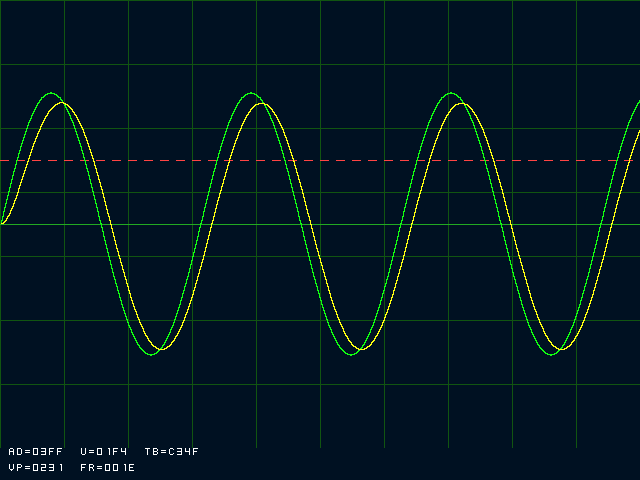
\includegraphics[width=0.78\linewidth]{../FPGA/src/vga/preview_640x480.png}
\caption{640$\times$480 显示效果（按 RTL 相同的映射关系复现）：双通道波形、64$\times$64 网格、
零电平轴、红色虚线为触发电平，底部两行为运行值。}
\label{fig:scope-preview}
\end{figure}

已知限制：（1）触发为“指针归零”式对齐，没有预触发深度与单次捕获；
（2）频率由帧内过零数 $\times$60 得到，分辨率 60Hz，且阈值固定为 512；
（3）滚动模式每帧更新一次基准，极高采样率下帧间会有跳变；
（4）串口命令为 ASCII 文本，极端情况下可能与二进制帧混淆；
（5）文本为固定模板，暂不支持任意字符串。
